% !TEX root = 99_main.tex

To study the electricity generation and building energy consumption, a 3D geometry of the room and solar facade is built using the Rhinoceros software \cite{Rhino}, and its parametric modelling plugin Grasshopper \cite{grasshopper}. The solar facade consists of 400mm CIGS square panels that can rotate in two degrees of freedom. On the horizontal axis, the panels can move from 0$^{\circ}$ (closed) to 90$^{\circ}$ (open) position in steps of 22.5$^{\circ}$. In the vertical axis, it can move from 45$^{\circ}$ to -45$^{\circ}$ in 22.5$^{\circ}$ steps. Existing ASF systems \cite{nagy2015frontiers} have independently actuated panels and a continuous range of actuation, however for simplicity, we group all panels into one cluster that moves in unison. This leaves us with 25 possible dynamic configurations of the facade system. A corresponding workflow can be seen in Figure \ref{fig:workflow}. 

\subsection{Building Energy Demand}

The building energy simulation is conducted using EnergyPlus \cite{energyplus} through the DIVA \cite{DIVA} interface. A summary of the energy simulation parameters can be found in Table \ref{tab:AssumptionsOpp}. The geometric solar facade is interpreted in EnergyPlus as an external shading system. A simulation of each possible dynamic configuration of the facade is run for each hourly timestep of the year using using a weather file for Zurich, Switzerland [REF REQUIRED].

\begin{table*}
\centering
\begin{tabular*}{\textwidth}{ll}
\hline
\textbf{Building Settings}    &                                                \\
Office Envelope               & Roof: Adiabatic                                \\
                              & Floor: Adiabatic                               \\
                              & Walls: Adiabatic                               \\
                              & Window: Double Glazed (e=0.2) 3mm/13mm air \\
Thermal Set Points            & Heating: 22$^{\circ}$C          \\
                              & Cooling: 26$^{\circ}$C          \\
Building System               & Hydronic Heating: COP=4                        \\
                              & Hydronic Cooling: COP=3                        \\
Lighting Control              & Lighting Load: 11.8W/m$^2$                                  \\
                              & Lighting Control: 300 lx Threshhold            \\
Occupancy                     & Office: Weekdays from 8:00-18:00               \\
                              & People set point: 0.1 persons/m$^2$               \\
							& Ventilation: 0.0094 m$^3$/s/person               \\
                              & Infiltration: 0.5 air changes per hour                     \\
                              &                                                \\
\textbf{Location Assumptions} &                                                \\
Weather File                  & Zurich Kloten, Switzerland                \\
\hline
\end{tabular*}
\caption{Summary of main assumptions for the calculation of operational emissions}
\label{tab:AssumptionsOpp}
\end{table*}

\subsection{PV Electricity Supply}

A solar radiance simulation is run in parallel using Ladybug \cite{roudsari2014ladybug},  which uses Radiance \cite{ward1994radiance} to determine the incident insolation on the solar facade. The approach enables us to calculate solar irradiance on the modules with high spatial resolution including the effect of module mutual shading as seen in Figure \ref{fig:radiation}. The results are coupled to an electrical circuit simulation of thin-film PV modules with sub-cell level representation \cite{hofer2015PVSEC}. 

\textcolor{magenta}{@Jeri, can you add a paragraph here about how the electrical simulation in python works}

This enables us to also account for losses in module efficiency through self shading.

\subsection{Optimisation}
Results of the PV Electricity Supply, and Building Energy Demand for each possible configuration of the ASF, for each timestep is imported into Python \cite{python} for post processing. The optimum configuration that minimises building energy consumption, and maximumised PV electricity production is calculated for each hourly timestep. 



\begin{figure}
\begin{center}
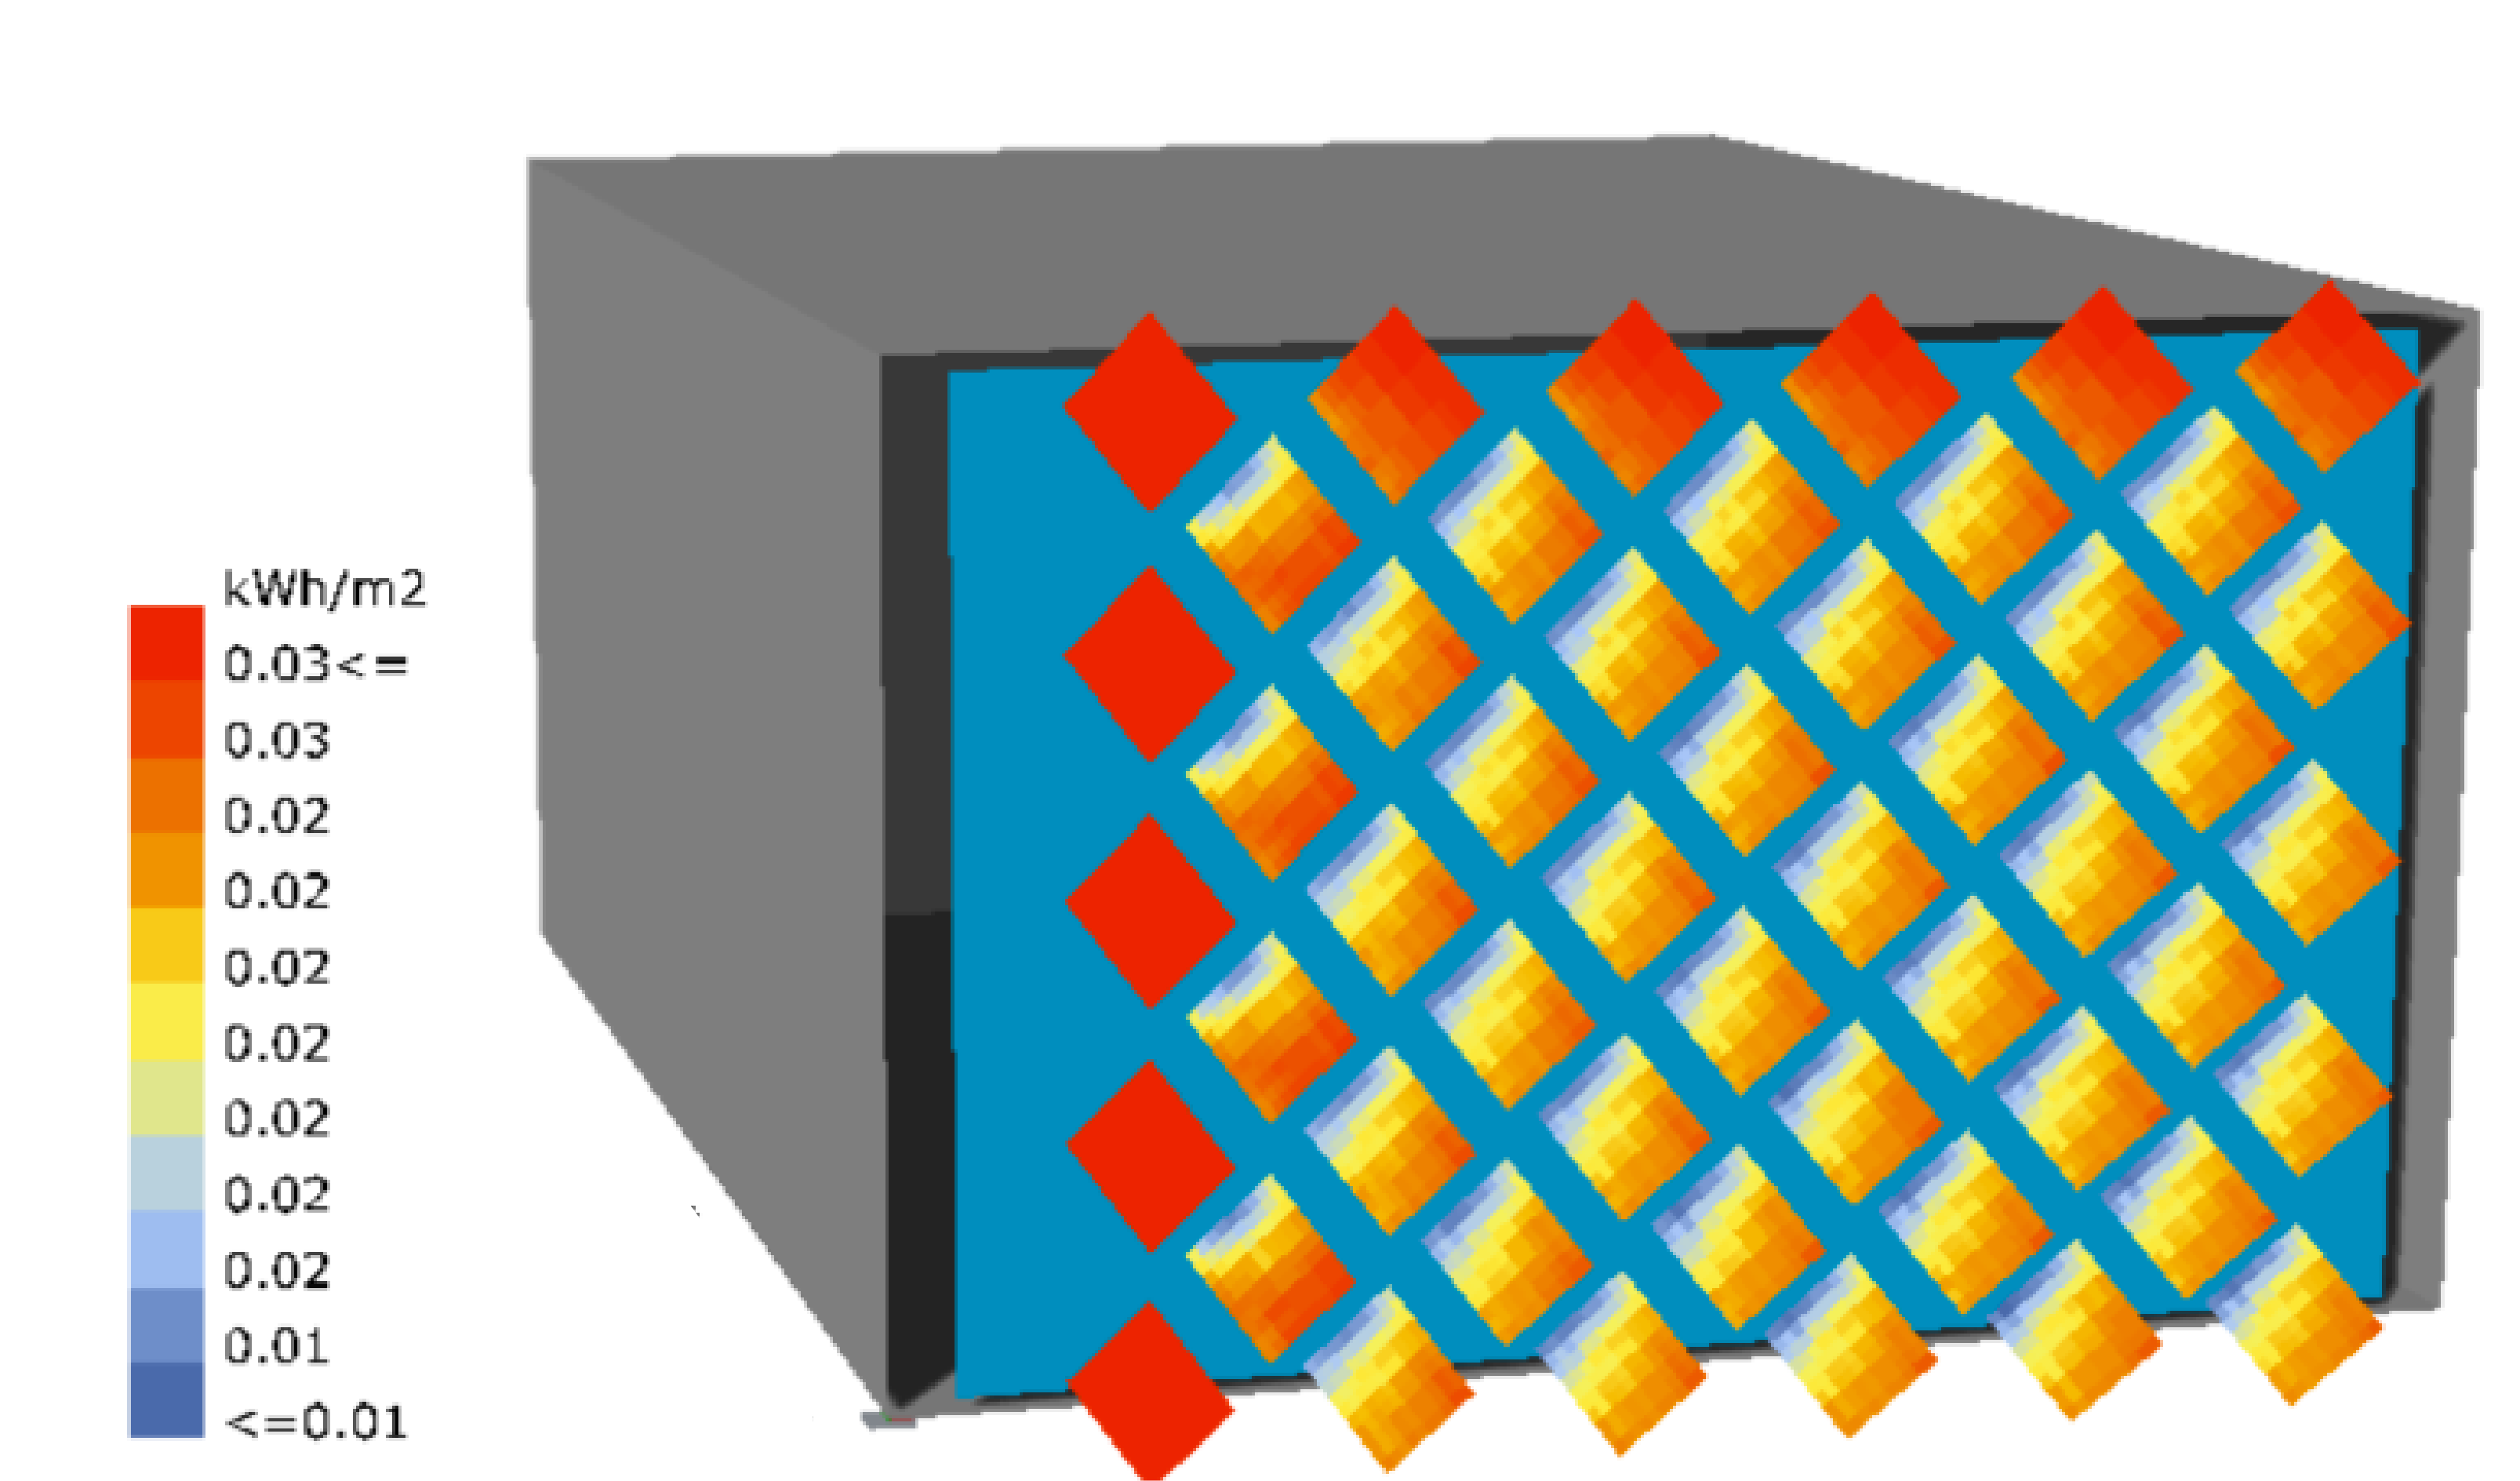
\includegraphics[width=8cm, trim= 0cm 0cm 0cm 0cm,clip]{radiationanalysis.png}
\caption{A simulation result showing module insolation from 11:00-12:00 on the 16 June for the used weather file and a specific module orientation.}
\label{fig:radiation}
\end{center}
\end{figure}


\begin{figure}
\begin{center}
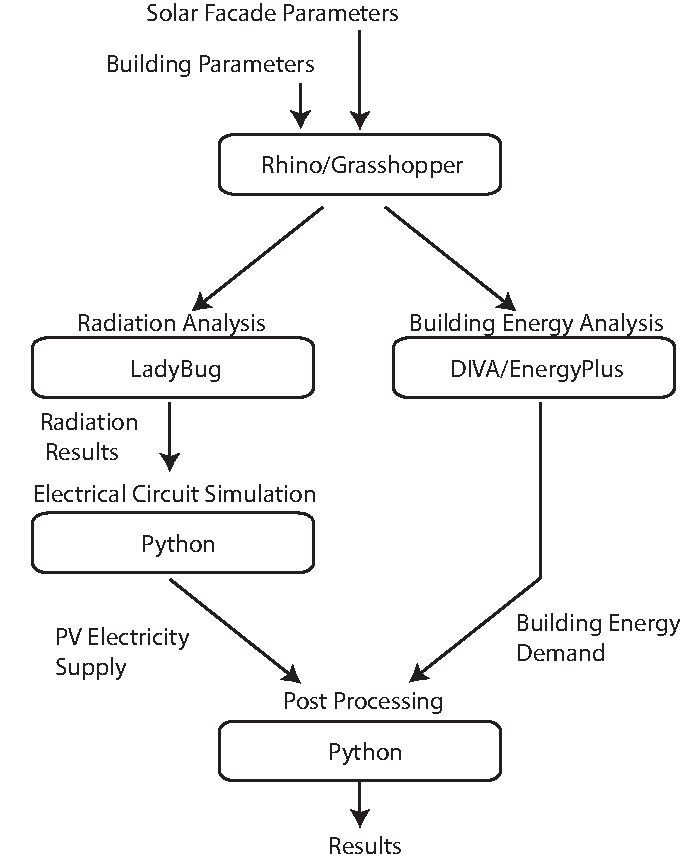
\includegraphics[width=\columnwidth, trim= 0cm 0cm 0cm 0cm,clip]{workflow_vertical.pdf}
\caption{Simulation Workflow}
\label{fig:workflow}
\end{center}
\end{figure}

\subsection{Sensitivity Analysis}
(optional)
A sensitivity analysis was conducted to determine the effects of 

\begin{itemize}
\item The location of operation. Madrid and Singapore
\item The office parameters. A building with a higher infiltration (1 air change per hour) and ventilation rate (0.016 m$^3$/s/person)
\item The efficiency of the cooling system (COP=7)